
\chapter{Преглед коришћених симбола у блок дијаграмима} \label{a:blok}

\subsection*{Основне шематске ознаке}

\noindent
\begin{tabular}{ll}
    \begin{minipage}{0.1\textwidth}
        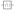
\includegraphics[page=1]{fig/standard.pdf}     
    \end{minipage}
    & 
    \begin{minipage}{0.8\textwidth}
        Систем, без меморије, представљен функцијом преноса $y = f(x)$.
    \end{minipage}
    \\[5mm]
    \begin{minipage}{0.1\textwidth}
        \includegraphics[page=2]{fig/standard.pdf}     
    \end{minipage}
    & 
    \begin{minipage}{0.8\textwidth}
        Систем представљен оператором $\rm L$. 
    \end{minipage}
    \\[5mm]
    \begin{minipage}{0.1\textwidth}
        \includegraphics[page=3]{fig/standard.pdf}     
    \end{minipage}
    & 
    \begin{minipage}{0.8\textwidth}
        Систем представљен својим импулсним одзивом, $h = h(t)$ односно\linebreak $h = h[n]$.
    \end{minipage}
    \\[5mm]
    \begin{minipage}{0.1\textwidth}
        \includegraphics[page=4]{fig/standard.pdf}     
    \end{minipage}
    & 
    \begin{minipage}{0.8\textwidth}
        Интегратор, $y(t) = \int_{\mathclap{-\infty}}^{\mathclap{t}} x(\uptau) \, \de\uptau$,
        са нултим почетним условом.
    \end{minipage}
    \\[5mm]
    \begin{minipage}{0.1\textwidth}
        \includegraphics[page=15]{fig/standard.pdf}     
    \end{minipage}
    & 
    \begin{minipage}{0.8\textwidth}
        Акумулатор, $y[n] = \sum_{\mathclap{m = -\infty}}^{n} x[m]$,
        са нултим почетним условом.
    \end{minipage}
    \\[5mm]
    \begin{minipage}{0.1\textwidth}
        \includegraphics[page=5]{fig/standard.pdf}     
    \end{minipage}
    & 
    \begin{minipage}{0.8\textwidth}
        Диференцијатор, $y(t) = \dfrac{\de x(t)}{\de t}$. 
    \end{minipage}
    \\[5mm]
    \begin{minipage}{0.1\textwidth}
        \includegraphics[page=6]{fig/standard.pdf}     
    \end{minipage}
    & 
    \begin{minipage}{0.8\textwidth}
        Идеални појачавач. Појачање се може уписати у симбол. 
    \end{minipage}
    \\[5mm]
    \begin{minipage}{0.1\textwidth}
        \includegraphics[page=7]{fig/standard.pdf}     
    \end{minipage}
    & 
    \begin{minipage}{0.8\textwidth}
        Блок за кашњење, $y(t) = x(t-\uptau)$. 
    \end{minipage}
    \\[5mm]
    \begin{minipage}{0.1\textwidth}
        \includegraphics[page=8]{fig/standard.pdf}     
    \end{minipage}
    & 
    \begin{minipage}{0.8\textwidth}
        Дискретан блок за кашњење, $y[n] = x[n - N]$. 
    \end{minipage}
\end{tabular}

\noindent
\begin{tabular}{ll}
    \begin{minipage}{0.1\textwidth}
        \includegraphics[page=9]{fig/standard.pdf}     
    \end{minipage}
    & 
    \begin{minipage}{0.8\textwidth}
        Сабирач, са произвољним улазним предзнаком сигнала, $z = \pm x \pm y$.
    \end{minipage}
    \\[5mm]
    \begin{minipage}{0.1\textwidth}
        \includegraphics[page=10]{fig/standard.pdf}     
    \end{minipage}
    & 
    \begin{minipage}{0.8\textwidth}
        Множач/миксер/модулатор, $z(t) = K ( x(t)\cdot y(t))$, $K = \const$.
    \end{minipage}
\end{tabular}

\subsection*{Фреквенцијски селективни филтри}

\noindent
\begin{tabular}{ll}    
    \begin{minipage}{0.1\textwidth}
        \includegraphics[page=11]{fig/standard.pdf}     
    \end{minipage}
    & 
    \begin{minipage}{0.8\textwidth}
        Филтар пропусник ниских учестаности (НФ). 
    \end{minipage}
    \\[5mm]
    \begin{minipage}{0.1\textwidth}
        \includegraphics[page=12]{fig/standard.pdf}     
    \end{minipage}
    & 
    \begin{minipage}{0.8\textwidth}
        Филтар пропусник опсега учестаности (ПО).
    \end{minipage}
    \\[5mm]
    \begin{minipage}{0.1\textwidth}
        \includegraphics[page=13]{fig/standard.pdf}     
    \end{minipage}
    & 
    \begin{minipage}{0.8\textwidth}
        Филтар пропусник високих учестаности (ВФ). 
    \end{minipage}
    \\[5mm]
    \begin{minipage}{0.1\textwidth}
        \includegraphics[page=14]{fig/standard.pdf}     
    \end{minipage}
    & 
    \begin{minipage}{0.8\textwidth}
        Филтар непропусник опсега учестаности (НО).
    \end{minipage}
\end{tabular}

% \begin{figure}[ht!]
%     \begin{subfigure}[c]{0.32\textwidth}
%         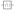
\includegraphics[page=1]{fig/standard.pdf}
%         \caption{Систем представљен статичком функцијом преноса $y = f(\cdot)$}
%     \end{subfigure}
%     %
%     \begin{subfigure}[c]{0.32\textwidth}
%         \includegraphics[page=2]{fig/standard.pdf}
%         \caption{Систем представљен оператором $y = f(\cdot)$}
%     \end{subfigure}
% \end{figure}